\documentclass[conference]{IEEEtran}
\IEEEoverridecommandlockouts
% The preceding line is only needed to identify funding in the first footnote. If that is unneeded, please comment it out.
\usepackage{amsmath,amssymb,amsfonts}
\usepackage{algorithm}
\usepackage{algpseudocode}
\usepackage{graphicx}
\usepackage{textcomp}
\usepackage{xcolor}
\usepackage[english]{babel}
\usepackage{biblatex}
\addbibresource{sample.bib}
\def\BibTeX{{\rm B\kern-.05em{\sc i\kern-.025em b}\kern-.08em
    T\kern-.1667em\lower.7ex\hbox{E}\kern-.125emX}}
\begin{document}

\title{An introduction to stochastic multi-armed bandits}

\author{\IEEEauthorblockN{1\textsuperscript{st} Sheel Shah}
\IEEEauthorblockA{\textit{Department of Electrical Engineering} \\
\textit{IIT Bombay}\\
Mumbai, India \\
19D070052@iitb.ac.in}
}

\maketitle

\begin{abstract}
This paper aims to provide an overview of the stochastic multi-armed bandit problem and describe renowned algorithms that solve the problem. The multi-armed bandit (MAB) setting has been attracting the attention of scholars from a broad spectrum of fields, with its several variants having applications in a wide range of problems. This paper also describes a few of these variants and state-of-the-art approaches to solving them.
\end{abstract}

\section{Introduction}
The multi-armed bandit problem inherits its name from slot machines, where one pulls an "arm" to obtain some (monetary) "reward". A single slot machine is referred to as a "one-armed bandit", and a multi-armed bandit is analogous to several slot machines in a row. A rational person wants to obtain as much reward as he can, but since he is restricted by how many times he can play at the slot machines, he must identify and play the machine that, on average, provides the most reward.

This setup abstracts the fundamental problem of trading off between exploration — the search for new good options and exploitation — using what has already been learnt. Reference \cite{bandit_intro} first introduced this idea of the \textit{exploration versus exploitation tradeoff} in sequential decision problems, and a plethora of work has followed since. A few applications that motivate the study of multi-armed bandits are: 
\begin{itemize}
    \item \textbf{A/B Testing}\cite{ab_testing}: When deciding between several variations of the same feature in some user-based product, each variant can be abstracted as an arm of the bandit with some positive reward associated based on the user's experience when interacting with this feature.
    \item \textbf{Medical Trials}\cite{medical_testing}: Determining the effectiveness of different medicines against a disease can also be modelled as a multi-armed bandit problem. Since human trials are expensive and difficult to conduct, we want to determine the "best" medicine using as few trials as possible.
\end{itemize}

The rest of this paper is structured as follows: In section II, the exact problem of (stochastic) multi-armed bandits is formalized as per convention in the literature. Section III overviews two classic algorithms — KL-UCB and Thompson Sampling. Section IV describes some variants of the simple stochastic bandit and briefly discusses popular approaches used. Finally, section V talks about the state of the theory and future work in this domain.

\section{The multi-armed bandit model}
We first introduce the notion of the "environment" and the "player". The player is a decision-making entity that \textit{interacts} with the environment. Particularly, the environment consists of bandit arms and their reward functions along with other quantities such as the number of arm-pulls that the player, in total, is allowed to make; and the player aims to maximize the net reward. The interaction here is the pulling of arms and the reception of reward drawn from the corresponding reward function. It is important to note that the player does not have direct access to environment objects because, otherwise, the problem of maximizing net reward is trivial.

Hence in each time step, the player chooses an arm to pull and sees a reward drawn from the corresponding reward function. The choice of the pulled arm, as is intuitive, can only be based on the history of interactions seen so far.

The following notation is used throughout the rest of this paper:
\begin{align*}
    K &= the\ number\ of\ arms\ of\ the\ bandit\\
    X_i &= the\ random\ reward\ associated\ with\ arm\ i\\
    H &= horizon;\ the\ number\ of\ pulls\\
    S_t &= the\ arm\ pulled\ by\ the\ player\ at\ time step\ t\\
\end{align*}
In the stochastic setting, $K$ is considered to be finite, and the functions $X_i$ stationary (i.e. time-invariant). Most results discussed subsequently are in the limit $H \to \infty$, but similar empirical results are seen in practice for finite $H$.

Whilst the introduction discussed \textit{maximizing} net reward, the convention followed is to \textit{minimize} regret. Both these objectives are equivalent. We define the expected-expected regret as follows:
\begin{align*}
    R &= \sum_{t=1}^H (E[X^*] - E[X_{S_t}])\\
    where\ X^* &= arg\max_{i \in [K]} E[X_i]
\end{align*}

A seminal paper by Lai and Robbins \cite{lai_robbins} proved that for the previously discussed constraints, if a player achieves sub-linear regret for all bandit instances, then for every non-trivial bandit instance:
\begin{equation*}
    \liminf_{H \to \infty} \dfrac{R}{ln\ H} \geq \sum_{i: E[X_i] < E[X^*]} \dfrac{E[X^*] - E[X_i]}{D(X_i, X^*)}
\end{equation*}
Here, one particular set of arms and reward distributions is referred to as a bandit instance, but there are no other assumptions whatsoever (which is what makes this limit a fundamental one in the study of MABs). D is the Kullback-Leibler divergence \cite{KL_divergence} between reward distributions. In essence, \textit{sub-logarithmic regret cannot be achieved} by any "good" algorithm.


Other standard multi-armed bandit settings and regret definitions can be found in \cite{lattimore_intro}.

\section{Optimal Algorithms}
\subsection{The UCB Algorithm}
\begin{algorithm}
\caption{The Upper Confidence Bound algorithm \cite{lattimore_ucb}}\label{alg:cap}
\begin{algorithmic}
\Require $H$, $K$
\State Pull each arm once, and initialize the reward history for each arm
\For{$t = 1, 2, ..., H$}
    \For{$i = 1, 2, ..., K$}
    \State $\hat{\mu_i}(t-1) \gets$ the empirical mean of arm $i$ upto time $t-1$
    \State $T_i(t-1) \gets$ the number of times arm $i$ is pulled upto time $t-1$
    \State $UCB_i(t-1) \gets \hat{\mu_i}(t-1) + 2\sqrt{\dfrac{log(n)}{T_i(t-1)}}$
    \EndFor
    \State Pull arm $S_t = arg\max_{i \in [K]} UCB_i(t-1)$
    \State Store the received reward in the reward history of arm $S_t$
\EndFor
\end{algorithmic}
\end{algorithm}

The UCB algorithm works on the principle of \textit{optmism under uncertainty}. A high-confidence bound of each arm's mean is computed, and the upper limit of this interval is used to decide the arm to be pulled next (hence, giving the algorithm its name). The exact form of the UCB is derived using the Chernoff-Hoeffding inequality \cite{chernoffhoeffdinginequality}, and it has been shown \cite{lattimore_ucb} that the above described UCB algorithm achieves regret of the form:
\begin{equation*}
    \lim_{H \to \infty} \dfrac{R}{ln\ H} \leq \sum_{i: E[X_i] < E[X^*]} \dfrac{16}{E[X^*] - E[X_i]}
\end{equation*}

UCB is thus is only a constant factor worse than the lower bound shown by Lai and Robbins.

\subsection{Thomspon Sampling}
We only discuss a particular version of Thompson Sampling (TS) in this section for brevity. The reward distribution of each arm is restricted to a Bernoulli distribution, and the prior (described next) used is a Beta distribution.

TS is a Bayesian algorithm, meaning it maintains a "belief" of the means of each arm, and this belief is updated whenever the player encounters new "evidence". The beliefs before and after the update are called the prior and the posterior, respectively. When new evidence is seen, the current posterior now becomes the prior. The posterior is calculated by Bayes' rule as:
\begin{equation*}
    posterior = \dfrac{prior\ *\ (likelihood\ of\ evidence)}{probability\ of\ evidence}
\end{equation*}

For the case of Bernoulli-armed bandits, we define our prior on the mean of arm $i$ as $Beta(\alpha_i, \beta_i)$. Applying Bayes' rule yields:
\begin{equation*}
    posterior = \begin{cases}
    Beta(\alpha_i, \beta_i + 1), \text{if reward of 0 is received}\\
    Beta(\alpha_i + 1, \beta_i), \text{if reward of 1 is received}
    \end{cases}
\end{equation*}

We can now state the TS algorithm.
\begin{algorithm}
\caption{Thompson Sampling for Bernoulli-armed bandits \cite{thompson_sampling}}\label{alg:cap}
\begin{algorithmic}
\Require $K$
\State $\alpha_i \gets 1\ \forall i \in [K]$
\State $\beta_i \gets 1\ \forall i \in [K]$
\For{$t = 1, 2, ..., H$}
    \For{$i = 1, 2, ..., K$}
    \State Draw random $\hat{X}_i \sim Beta(\alpha_i, \beta_i)$
    \EndFor
    \State Pull arm $S_t = arg\max_{i \in [K]} \hat{X}_i$
    \State Receive reward $r$
    \If{$r = 1$}
    \State $\alpha_{S_t} = \alpha_{S_t} + 1$
    \Else
    \State $\beta_{S_t} = \beta_{S_t} + 1$
    \EndIf
\EndFor
\end{algorithmic}
\end{algorithm}

Thompson Sampling has the following regret guarantee:
\begin{equation*}
    \lim_{H \to \infty} \dfrac{R}{ln\ H} \leq \sum_{i: E[X_i] < E[X^*]} \dfrac{2}{E[X^*] - E[X_i]}
\end{equation*}

Hence, TS is optimal to the constant in the long run.

\begin{figure}[H]
    \centering
    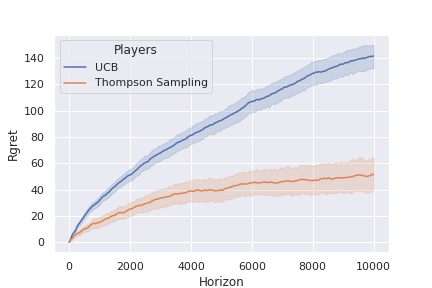
\includegraphics[width=8.8cm]{plot.png}
    \caption{The regret versus horizon plots for UCB and TS. The algorithms were tested against a Bernoulli-armed bandit with three arms of means 0.5, 0.67, 0.7. A total of 100 simulations were run per algorithm to abate the effect of randomization. The logarithmic nature of the regret is clearly visible, and UCB's regret being a constant factor worse is also apparent.}
    \label{fig:my_label}
\end{figure}

\section{Complications of multi-armed bandits}
There are several assumptions in the above-presented model of a stochastic multi-armed bandit. The following are some variants of the multi-armed bandit problem:
\begin{itemize}
    \item \textbf{Non-stationary MABs}: An instrumental assumption in the stochastic setting is the stationarity of the reward distributions of the arms. This model allows for gradual changes in the distribution and is more applicable to real-life scenarios where trends often slowly shift. Algorithms designed for the stationary setting do not generally perform well under this model, but Thompson sampling can be modified into non-stationary Thompson sampling \cite{thompson_sampling} to handle time-varying reward distributions.
    \item \textbf{Adversarial bandits}: As the name suggests, this model is \textit{adversarial} to the player. An adversary now picks the reward distributions, and the player is unaware of this choice. The adversary is considered to have access even to the player's strategy. Deterministic algorithms are entirely useless in this setting, and we must, hence, randomize our algorithms. For our analyses to have meaning, a different form of regret called "weak-regret" is analysed, under which the Exp3 algorithm \cite{exp3} achieves sub-linear regret.
    \item \textbf{Infinite-armed bandits}: This variant of the classic model treats the number of arms as an infinite or continuous range, with some method for discretizing the infinite space. By altering how much the agent knows about the arm-reward relationship, this version allows for significant variation in problem difficulty. This is better explained via an example. Consider the problem of picking the background color of a website to maximize its view time. This requires an underlying (random) funtion that maps the space of colors to the user's view time. One method to approach this problem is to treat the reward function as a smooth tree. The Bandit Algorithm for Smooth Trees \cite{bast} is a generalization of UCB combined with Monte Carlo Tree Search over infinite spaces.
    \item \textbf{Contextual bandits}: Contextual bandits are used for modelling extra information that we might have about arms. Given this information a priori, the player can learn about other arms without playing them. This additional information is usually represented as a \textit{feature}, and the reward is a function of this feature along with some unknown parameter. Reference \cite{contextual} introduces a contextual bandit algorithm that shows positive results in the scenario of personalized news article recommendations. News articles' features are extracted, and every person's personal choice of news forms the unknown parameter of the reward function.
\end{itemize}

\section{Conclusion}
Multi-armed bandits have been extensively studied because of how well they model the exploration/exploitation dilemma and how easily they can be tweaked to be applicable in real scenarios, replacing traditional methods that rely on the storage of lots of data. The algorithms discussed in this paper can be modified to avoid having to store the history of rewards and store empirical means instead, making them \textit{truly online}.

The primary metric used throughout this paper has been regret (expected-expected regret to be precise), but the literature also includes other measures of the performances of algorithms. Instead of reward maximization (and equivalently, regret minimization), another definitive objective is best-arm identification. The aim under best-arm identification is to explore as well as possible, and exploitation is not considered. The player attempts to find an arm that is optimal with high probability under some horizon constraint. The idea can be generalized to best-K identification.

Most common algorithms have high-confidence bounds on the optimal arm but lack much information about other arms other than their sub-optimality. Methods to correctly bound all arms might be explored in the future. One might also study regret-based performance guarantees of existent algorithms under inconsistent reward distributions across arms.
\printbibliography

\end{document}

